% ------------------------------------------
%  MASTER THESIS DISSERTATION
% ------------------------------------------
% Author:
%
% Advisors:
%
% ------------------------------------------
\documentclass[10pt,twoside,a4paper]{report}
% Set document margins to 1in in all sides
\usepackage[margin=2.5cm]{geometry}
% Line spacing package
\usepackage{graphicx, helvet, hyperref, inputenc, setspace}
\usepackage[portuguese,english]{babel}
\usepackage[acronym]{glossaries}
\usepackage{tabulary}
%\usepackage{tikz}
\usepackage{pgfplots}
\usepackage[simplified]{pgf-umlcd}
\usepackage{listings}
\usepackage{array}

\lstdefinestyle{customhtml}{
  language=HTML,
  showstringspaces=false,
  basicstyle=\footnotesize\ttfamily,
  keywordstyle=\bfseries\color{green!40!black},
  commentstyle=\itshape\color{purple!40!black},
  identifierstyle=\color{blue},
  stringstyle=\color{orange},
  tabsize=2
}

\definecolor{javared}{rgb}{0.6,0,0} % for strings
\definecolor{javagreen}{rgb}{0.25,0.5,0.35} % comments
\definecolor{javapurple}{rgb}{0.5,0,0.35} % keywords
\definecolor{javadocblue}{rgb}{0.25,0.35,0.75} % javadoc
\definecolor{javaStringBlue}{rgb}{0.1647,0,1}

\lstdefinestyle{customjava}{
language=Java,
basicstyle=\footnotesize\ttfamily,
keywordstyle=\color{javapurple}\bfseries,
stringstyle=\color{javaStringBlue},
commentstyle=\color{javagreen},
morecomment=[s][\color{javadocblue}]{/**}{*/},
tabsize=4,
showspaces=false,
showstringspaces=false
}

% Built the glossary when the main file is built.
\makeglossaries
% Set main font to Arial
\renewcommand{\familydefault}{\sfdefault}
% Define keywords macro
\providecommand{\keywords}[1]{\textbf{Keywords:} #1}
% Section numbering depth
\setcounter{secnumdepth}{2}
% Table of contents depth
\setcounter{tocdepth}{3}
% Set line spacing to 1.5cm
\onehalfspacing
% Page numbering
\pagestyle{plain}

% Glossary-File
% Glossary Definition

\newglossaryentry{MSc}{name={MSc}, description={Masters degree in the area of Science.}}

% Acronym-File
% Acronym Definition

\newacronym{IST}{IST}{Instituto Superior T\'ecnico}


% ------------------------------------------
% MASTER THESIS DISSERTATION
% ------------------------------------------

\begin{document}
%!TEX root = ./dissertation.tex

% Dissertation basic information
\newcommand {\Title} {Collaborative Platform for Analysis of Software Systems}
%\newcommand {\Subtitle} {My Subtitle}
\newcommand {\StudentName} {Catarina Isabel Carvalho Santana}
\newcommand {\DegreeName} {Information and Software Engineering}
\newcommand {\Supervisors} {Prof. António Manuel Ferreira Rito da Silva}

% Include or not include acknowledgments
\def \includeAcknowledgments{1}

% Include or not include glossary
\def \includeGlossary{0}

% Examination Committee
\newcommand {\Chairperson} {Prof./Dr. Lorem Ipsum}
\newcommand {\Advisor} {Prof./Dr. António Manuel Ferreira Rito da Silva}
\newcommand {\CommitteeMembers} {Prof./Dr. Lorem Ipsum}

% Date
\newcommand {\Month} {October}
\newcommand {\Year} {2015}

% You can define your own variables here


%!TEX root = ./dissertation.tex

% ---------------------------------------------------------
%   MASTER THESIS DISSERTATION COVER
% ---------------------------------------------------------
\begin{titlepage}
% ---------------------------------------------------------
%  INSTITUTION LOGO
% ---------------------------------------------------------

\includegraphics[width=5cm]{images/Logo_IST_color}~\\[2.0cm]
\begin{center}
% ---------------------------------------------------------
%  MASTER THESIS DISSERTATION TITLE
% ---------------------------------------------------------
{\LARGE \textbf{\Title}}\\[1.0cm]
% ---------------------------------------------------------
%  MASTER THESIS DISSERTATION SUBTITLE
% ---------------------------------------------------------
%{\Large \Subtitle}\\[1.0cm]
% ---------------------------------------------------------
%  AUTHOR NAME (FULL)
% ---------------------------------------------------------
{\Large \textbf{\StudentName}}\\[1.0cm]
% ---------------------------------------------------------
%  DISSERTATION DEGREE
% -----------------------------------------------------------------
{\large Thesis to obtain the Master of Science Degree in}\\[1.0cm]
% -----------------------------------------------------------------
%  COURSE NAME
% -----------------------------------------------------------------
{\LARGE \textbf{\DegreeName}}\\[1.0cm]

% -----------------------------------------------------------------
%  ADVISORS NAME
% ---------------------------------------------------------
\begin{minipage}[t]{.75\textwidth}
\begin{center}
{\large Advisor:\:}
{\Supervisors}
\end{center}
\end{minipage}\\[1.0cm]

% ---------------------------------------------------------
%  JURI NAMES:
%  - PRESIDENT
%  - ADVISOR
%  - VOGALS
% ---------------------------------------------------------


%{\Large \textbf{Examination Committee}}\\[.25cm]
%\begin{minipage}[t]{.5\textwidth}
%  \begin{flushright}
 %   {\large Chairperson:\:}\\
  %  {\large Advisor:\:}\\
   % {\large Members of the Committee:\:}
%  \end{flushright}
%\end{minipage}%
%\begin{minipage}[t]{.5\textwidth}
 % \begin{flushleft}
 %   {\Chairperson}\\
 %   {\Advisor}\\
 %   {\CommitteeMembers}
 % \end{flushleft}
%\end{minipage}\\[1.0cm]

% ---------------------------------------------------------
%  DATE (MONTH AND YEAR)
% ---------------------------------------------------------
{\Large \textbf{\Month\:\Year}}\\
\end{center}
\end{titlepage}


\if\includeAcknowledgments 1
%!TEX root = ../dissertation.tex

% Acknowledgments: This one is optional
\chapter*{Acknowledgments}


\fi
%!TEX root = ../dissertation.tex
\chapter*{}


``In the end, I'm able to look back without shame or regretful nostalgia and think, \textit{You did something great. And something new will come around. Or not. Either way, do the work you love. And love yourself. That's all you can do in this world in order to be happy}'' 

- Felicia Day in \textit{``You're Never Weird on the Internet (Almost)''}
%!TEX root = ../dissertation.tex

\begin{otherlanguage}{english}
\begin{abstract}
The Software Architectures course at Instituto Superior T\'{e}cnico teaches students the most important concepts on design and architecture of software systems and helps students to apply these concepts to real and complex software systems. Organizing knowledge and applying theory to practice is not an easy task, and students often need to ask questions and discuss. State-of-the-art on collaborative, social software and knowledge structuring was analyzed and a social platform was developed to help solving these problems.

% Keywords
\begin{flushleft}

\keywords{social software, knowledge structuring, collaborative platform, reputation systems, tagging systems, ontology, taxonomy}

\end{flushleft}

\end{abstract}
\end{otherlanguage}

%!TEX root = ../dissertation.tex

\begin{otherlanguage}{portuguese}
\begin{abstract}
O teu resumo aqui...

% Keywords
\begin{flushleft}

\keywords{as tuas palavras chave}

\end{flushleft}

\end{abstract}
\end{otherlanguage}


\tableofcontents
\listoftables
\listoffigures
\printglossary[type=\acronymtype]

%!TEX root = ../dissertation.tex

% Entry point for chapters
% In this file you define the order
% in which the chapters are included

% Chapters
%!TEX root = ../dissertation.tex

\chapter{Introduction}
\label{chapter:introduction}

NEEDS MOAR WORK.

Analyzing and discussing big, real, open-source and highly complex software system is a very important part of the Software Architectures course. In the course context, students must apply concepts and techniques for design and analysis of software architectures to descriptions of real systems. 

However, applying these concepts and techniques is not a very easy task, and often students have questions and doubts regarding these descriptions. These questions sometimes require not only consulting the course bibliography, but also discussing with peers or asking questions to teachers.

The following document is organized as follows: Section \ref{objectives} provides a more detailed description of the problem presented last paragraph and presents a possible solution for the problem. Section \ref{related} presents the state-of-the-art on the components of the solution. Section \ref{solarch} describes a possible solution for the problem and Section \ref{assessm} describes how the implemented solution will be assessed.

%TEX root = ../dissertation.tex

\section{Problem Description}
\label{chapter:problemdescription}
The course of Software Architectures at Instituto Superior T\'{e}cnico teaches students the most important concepts in the field of software architectures and applies these concepts to real-life software systems.

The practical component of this course (where the theory is applied) is done by analyzing documents/articles that describe the architectures of real-life systems and applying the concepts learned in theory lessons.
This analysis is either done by students with the help of the teacher, during practical classes, or in work groups of usually three students, that read, discuss and analyze software descriptions together and present their results to both the teacher and the rest of the class.

Understanding the analysis done and how it was done is very important, since it means students can apply the concepts learned not only in the written exam to pass the course, but also in the future, in other real-life software systems.

However, there are several issues regarding the application of theory concepts in this course:
\begin{itemize}
\item Each year, there are around one-hundred students signed in the course. All these students have roughly the same Computer Science background knowledge. However, not all students have the same maturity: while some may quickly understand what is taught in theory lessons, others may need some more time to assimilate what was taught.

\item The output of the analysis done to software descriptions (the scenarios, etc. extracted) is not available in a consistent way: the analysis done in class is available for students if they took their own notes, and the analysis done by groups is available if:
\begin{enumerate}
\item Students took notes of their colleagues' presentations 

\item Groups share their presentation slides among them. Slides may include errors pointed out by the teacher, but not corrected.
\end{enumerate} 

\item The case description is usually a fairly long document (from ten to twenty pages approximately). The task of carefully reading and understanding all the text and do a mapping between the concrete descriptions in the text and the abstract concepts learned in theory classes is not easy, as the parts of the text that map to concepts are not always evident.

\item The architectural elements extracted from a single software description are usually scattered along the whole text, and it is not evident the connection between all the elements.
\end{itemize}

%TEX root = ../dissertation.tex

\chapter{Objectives}
\label{chapter:objectives}
To solve the mentioned problems, we intend to develop a platform, where students and teachers collaborate in the analysis and synthesis of the case descriptions, ending on a structured representation of the case descriptions, that is hooked on the concrete description. 

The platform will provide ways for annotating the text on the case descriptions, which will help students organizing their thoughts and creating the structure. 

To motivate the students to participate in this platform and to increase the collaborative component, elements of social software will be used (such as reputation and tagging systems), to promote, among other things, collaboration, mutual aid, discussion, learning, and even some healthy competition between students.

 
The existence of this collaborative platform provides not only a way for students to discuss, ask questions and consolidate their knowledge, but also a unique place where their study materials are stored and organized, facilitating their studies.

%TEX root = ../dissertation.tex

\chapter{Related Work}
\label{chapter:relatedwork}
\label{related}
The platform to develop can be thought of a social software, where different people communicate and collaborate to provide a structured representation of a software description.
The next subsections provide an overview on the state-of-the-art of two main aspects:
\begin{itemize}
\item \textbf{Collaborative work}, presenting the state-of-the-art on social and collaborative aspects of software. This includes literature on:
	\begin{itemize}
		\item The Honeycomb Framework (a framework that generalizes the most important components of social software);
		\item Persuasive Software (systems that have impact on users behavior and thoughts, which is the case of the platform to develop);
		\item Roles in Social Networks (describing the types of users of social software);
		\item Reputation Systems (attribution of scores to users to provide a motivational component on the platform).
	\end{itemize}
	
\item \textbf{Knowledge Structuring}, presenting the state-of-the-art on ways of structuring information. This includes literature on:
	\begin{itemize}
		\item Collaborative tagging systems (assigning keywords to documents or parts of documents);
		\item Semi-structured content (providing a way of structuring knowledge without such strict rules as, for example, an ontology or a taxonomy);
		\item Ontology Learning (extracting knowledge from text).
	\end{itemize} 
\end{itemize}


\subsection{Honeycomb Framework}
The term ``Social Software'' is used in very different contexts \cite{pereira2010social}, and therefore, there are different definitions for it, given by different authors \cite{shirky2005group,klamma2007social,kolko2007mobile,wiley2008tagging,chatti2007future}. 

The definition of Social Software as ``systems that allow people, in their particularities and diversity, to communicate (interact, collaborate, exchange ideas and information) mediating and facilitating any kind of social relationship and favoring the emergence of a collective wisdom and a bottom-up organization'' \cite{pereira2010social} applies to our collaborative platform, in the sense that it should allow a large number of students, with different personalities and opinions, to ask questions to their colleagues, give opinions, receive feedback, etc, in order to correctly identify the architectural elements in a description of a software system, and therefore reach a complete and correct analysis of that system. 

The Honeycomb Framework was proposed to illustrate the seven elements that give a functional definition for social software \cite{smith2007social}:
\begin{itemize}
\item \textbf{Identity:} the unique identifier of a user within the system;
\item \textbf{Presence:} resources that allow knowing if certain identity is online;
\item \textbf{Relationship:} way to determine how users can relate/are related to others;
\item \textbf{Reputation:} way of knowing the status of a user in the system;
\item \textbf{Groups:} possibility to form communities of users that have common interests;
\item \textbf{Conversation:} resources for communication among the users (synchronous and/or asynchronous);
\item \textbf{Sharing:} possibility of sharing objects that are important to the users (videos, images, etc);

\end{itemize}

The Identity appears at the center of the framework, because it is the most basic requirement of any social system.

Although this framework identifies the major elements of a social system, it does not, in fact, specifies whether a system is social or not, a software system may implement all of these elements and still not be social.

Analogously, a system can be social with just a couple of elements implemented. So far, the only way to know if a system is social is to check if it complies with the definition (or with one of them).

In the platform to develop it is possible to identify the following elements of the framework:


\begin{itemize}
\item \textbf{Identity:} The identity is the central element of the framework and it is essential to the platform, as each student is a unique person and, therefore, must have a unique identification inside the platform. Since each student has already got a unique student number inside the whole university, the student number should be used for identification. The name of the student should also be added for purposes of identification, since it helps other users knowing who are they communicating with (it is easier to know who a student is if his name is available).

\item \textbf{Reputation:} To assess the quality and relevance of the participations in the platform, a reputation system must be used, as discussed in \ref{repsys}.

\item \textbf{Groups:} One of the evaluation methods of the Software Architectures' course is the realization of group works, where students form work groups, and each group will have to identify architectural elements in a description of a software system. The notion of these work groups must be present in the platform, since each group is a restricted set of people that are working towards the same goal: Correctly understand and identify the architectural elements in the description. 

\item \textbf{Relationship:} Although there is already an implicit relationship inside the platform (all students are colleagues of each others), this relationship has a specialization. Since students are divided in work groups, students inside a work group have a different relationship – they are group colleagues, and this relationship must be differentiated. As the teacher will also be a member of the platform, the relationship student-professor must always be present as well: a student does not have the same kind of interactions he has with a colleague when interacting with a teacher – therefore this kind of relationship must be present in the platform.

\item \textbf{Conversation:} The existence of discussions around elements to add/already added to the platform provides a way of communication between the users.

\item \textbf{Sharing:} Within the discussions around elements, it should be possible to share different kinds of objects (articles, links, etc), since they may be helpful to understand or complement what is being discussed. Since there are groups inside the platform, there should be present different levels of sharing:

\begin{enumerate}
\item \textit{Group level:} Shared objects are only available for a single work group. 
This way, groups can share documents, links, etc., that are important for completing their assignments, or help understand the description document;

\item \textit{General level:} Documents are shared inside a discussion, an added element, or as an answer to a question asked, and are available to all students in the platform;
\end{enumerate}


\item \textbf{Presence:} Considering that all communications are asynchronous, the notion of presence is not strictly necessary in the platform. 
However, it could be added, as a feature, a visible list of people online (logged in the platform) – similar to the ones present in many discussion forums.
\end{itemize}

\subsection{Persuasive Software Design Patterns}
The term ``persuasive technology'' is used to describe computer systems that have an impact on user's thoughts and may even lead to changes in their behavior \cite{fogg2002persuasive,oinas2009persuasive}.

There are three different possible outcomes for a persuasive system:

\begin{itemize}
\item Reinforcement - making current attitudes resistant to change;
\item Changing Outcome - changes in a person's response to an issue;
\item Shaping outcome - formulate a pattern for a situation where one did not exist before \cite{oinas2008towards};
\end{itemize}

The main users of the collaborative platform to develop will be MSc students attending the 'Software  Architecture' course. Even though they are familiar with some of the terms used in the context of the course, new terms are introduced as the course progresses. This platform is persuasive in the sense that it must change the way its users will look at a description of a Software System: reading is not enough, it is necessary to relate what is read with the terms and concepts learned in the classes.
Therefore, the most important outcome for this platform is the Changing Outcome: When a description of a system is presented, the students most not only read it, but also relate it to the concepts learned and use the platform to try and extract the correct scenarios and views from it.

The concept of social influence shows that in daily activities, human beings often influence or are influenced by the actions of other people. One's opinion might be a reflection of someone else's opinion, which is also directly or indirectly influenced by cultural norms, mass media, social networks, etc \cite{mavrodiev2013quantifying}. Therefore, social influence is a change in one's behavior (or attitudes or beliefs), caused by external pressures \cite{guadagno2010preference}. 

In our context, we want the students to contribute to the platform. Either by adding new elements (scenarios, views), discussing the elements added by their colleagues, or asking/answering questions. 
The platform should provide a way to do this, by allowing: 
\begin{itemize}
\item Insertion and edition of new elements to the conceptual structure, done by any student;
\item Comments (and responses to comments) on an element inserted;
\item Discussion Forums and Q\&A systems
\end{itemize}


While some students will want to start contributing to the platform right away, some of them will not initially feel compelled to that. However, as their colleagues and friends add contributions, and since one's actions are somehow influenced by other people, these students may probably start contributing to the platform as well. Even in a social context, because people do not live in isolation, students may talk, ask/answer questions and discuss in person about the system being analyzed in the platform. The outcome of these social interactions may be a new, relevant, contribution to the platform.

Four design patterns are proposed for persuasive systems, in order to introduce social influence in software features: Social Learning and Facilitation (SLF), Competition (COM), Cooperation (COO) and Recognition (REC) \cite{oduor2014persuasive}. 

\subsubsection{Social Learning and Facilitation (SLF):}

The concept of Observational Learning, introduced by the Social Learning Theory, states that people's behavior and skills are augmented through the act of observing others \cite{bandura1977social}, whilst the concept of Social Facilitation states that people's awareness of being observed/evaluated by others also has an influence on their behaviors \cite{zajonc1965social}. Therefore, the Social Learning and Facilitation pattern has the main purpose of enabling and enhancing the design of software features that allow to visualize the presence of other people, with the motivation that it is easier for individuals to pursue their goals if there is a clear awareness of other people pursuing the same goal and facing the same issues \cite{oduor2014persuasive}. 

In the context of our collaborative platform, it is necessary to persuade the students to add contributions as they may, at first, not feeling confident enough to add their own contributions, whether they are new elements, comments, questions/answers, etc. The platform should provide a way to visualize the elements recently added or that are currently under discussion – as students see their colleagues contributing towards the same goal, they may want to add their own contribution.

Considering that the users of the platform will be students, the Social Learning should have more emphasis over the Social Facilitation. Students have different rhythms of learning, and sometimes a concept may not be correctly understood at first. Asking questions or discussing elements of the analysis will help in the correct assimilation of concepts, and therefore it must be encouraged.

The Social Facilitation comes in the sense that moderation is necessary: while students are encouraged to contribute and ask questions in order to learn, they should strive to add relevant comments and ask relevant questions, as their contributions are seen by everyone.

\subsubsection{Competition (COM):}
Human beings have a natural drive for competition. Therefore, it can be used as a social support guideline, to motivate users to adopt attitudes and behaviors \cite{oinas2009persuasive}. The Competition pattern has the main purpose of using competitive elements, such as ranks, scores and levels, that allow users to compare their performance with others, and adjust their target goals based on these. However, as some people might see competition as a motivational factor for improvement, other people may see it as a source of anxiety – therefore, participation in a competition must always be voluntary \cite{oduor2014persuasive}.

Adding competitive elements to a social system will, as said above, trigger the human being's natural drive for competition. Adding a score for each student and a rank hierarchy based on the range of scores will start a hopefully healthy competition between students. Each contribution should have a positive score, given either by the teacher or by the colleagues. Less correct contributions should have a lower score, but positive nonetheless. When a student adds something to the platform, it means that he is making an effort to apply the concepts learned in the classes. As said before, not all students can do this correctly at first, and therefore if one of them specifies an incorrect scenario, for example, it shouldn't have a negative score: trying and failing is a way of learning. In addition, when another student adds a contribution to correct his colleagues, he is also gaining score points, and therefore, increasing the competition.

Even this kind of competition, that is supposed to be healthy and motivating, can be a source of anxiety for some people. Therefore, it should be optional for students to be assigned a score and receiving points, or even to show their identity when contributing (add anonymity to the platform). 

\subsubsection{Cooperation (COO)}
Besides competition, reciprocity is also another human beings' natural drive \cite{cialdini1993influence,malone1987making}, and cooperation between people has been proven to cause positive impact on user behaviors \cite{stibe2012exploring}. The Cooperation pattern has the main purpose of providing software features that allow users to engage in mutual goals and provide ways for them, supporting each other in reaching their goals. The motivation for this pattern is that it is easier to cooperate if there is a clear awareness of what needs to be done, what other people are doing, and how far they are in achieving their goals. Group discussion supports these needs and encourages giving and receiving support on the matter. However, some people prefer to perform alone, and therefore cooperation must not be forced \cite{oduor2014persuasive}. 

The students that will use this platform will be working towards a main goal: correctly understanding and correlating what was learned in the Software Architectures classes with real examples of software systems. But concerning the analysis of a single software system, there are several concepts and structures to identify on a single description. Students may be having some trouble identifying these elements, and therefore the system must provide a way of defining goals. A goal, for example, could be ``Add a new scenario for Availability''. 

The goals system should work similarly to a discussion forum: Students can add, delete or change goals (changing the description or the title, for example), and for each goal it is possible to send messages to discuss it and ask or answer questions. As discussion around the goal progresses, students collaborate with each other by answering questions asked by their colleagues or correcting what some other student wrote before. Discussions can converge, then, to a correct identification of architectural elements in the platform. A goal should be able to be marked as ``in progress'' or ``complete'', to indicate that discussions around that goal are still in progress or have finished. 
Goals can also be split in sub-goals – if the discussion around a single goal becomes too big and complex, it might be wise to be able to split the discussion in sub-goals, each with its own discussion – so that when all sub-goals are complete, the main goal will also be nearly or fully complete. 

\subsubsection{Recognition (REC)}

In addition to competition and cooperation, recognition is introduced as another interpersonal motivational factor. This happens because people take pleasure in having their efforts recognized and appreciated by others, in order to feel fulfilled for their achievements \cite{malone1987making}. 
The Recognition pattern has the purpose of providing software features that enable users to get recognition from their peers. The motivation for this pattern is that users, when working towards a goal, they sometimes need a reason to focus on that same goal. Having their efforts recognized may be a good reason to keep the good work, and therefore systems should provide opportunities for public recognition of top achievers \cite{oduor2014persuasive}. 

As mentioned before, the users of this platform are students that are pursuing a Masters degree. And just like any other human being, students like to feel that their efforts are recognized. Not only recognition leads to a sense of fulfillment, but also it is a motivational factor to keep up the good work. 

Since the system should have a score system, this score should be used as a way of creating a weekly spotlight: by keeping track of the amount of points scored by each student along the week, as the week ends, the list of the Top 10 students with most points gathered in that week should be visible when entering the platform. The list of all students, in decreasing order of weekly points, could also be consulted.

Recognition is then achieved when students see their names in the spotlight. In addition to that, there may be some (hopefully healthy) competition for a spot in the Top 10 - as all, or at least most students will want to have their names on the spotlight.

\subsection{Roles in Social Networks}
A survey on the state-of-the-art regarding identification of roles in social networks (\cite{forestier2012roles}) starts by stating the difference between a ``role'' and a ``position'', by giving a definition for both of these concepts:
\begin{itemize}
\item A \textit{position} is a ``well-defined place'' of an individual in a social structure, and is usually associated with certain attitudes, mental health, knowledge, etc., of individuals \cite{forestier2012roles,borgatti1992notions}.
\item A \textit{role}, in a social structure, is a set of expectations for an individual in a certain position. For example, the role of ``secretary'' is associated to what secretaries are expected to do \cite{forestier2012roles,nadel1957theory}.
\end{itemize}
The survey divides the roles in two categories:
\begin{itemize}
\item \textit{Non-explicit roles}: roles that are not defined a-priori
\item \textit{Explicit roles}: predefined types of actors in the social network, such as ``experts'' or ``influencers''.
\end{itemize}

Methodologies for inferring \textit{non-explicit} roles analyze the structure of the social network and communications between users, in order to identify patterns in communication that allow the identification of roles. Common approaches are based on blockmodels \cite{borgatti1993two,breiger1975algorithm} and probabilistic bayesian models \cite{steyvers2004probabilistic,mccallum2007topic,daud2009generalized}.

Methodologies for identifying \textit{explicit} roles in a social network compare the activity of the user inside a social network against the criteria that characterizes each role. For example, techniques for identification of ``experts'' (users that answer correctly to questions asked) inside forums \cite{zhang2007expertise} analyze, among other criteria, the number of answers given by the user and how many different people a user answers.

In the platform to develop, it is possible to define a priori the two main roles:
\begin{itemize}
\item Student: it is the role assigned to most of the users. Students are the most active users, and their contributions to the platform include tagging parts of the document, adding and editing parts of the semi-structure, asking and answering questions and rate other students' contributions.


\item Teacher: this role is assigned to a very small number of users in the platform, but there must be at least one teacher present. Their number of contributions is smaller and they are mostly for correcting (through adding comments to the elements added, or answering questions) the contents added by the students to the platform. Teachers can also give ratings to the contents of the platform. It is up to the teachers to define the weight of their ratings on a case by case strategy.
\end{itemize}

The methodologies for identification of explicit roles in a social network \cite{zhang2007expertise,agarwal2008identifying} have in consideration social networks around the web, with hundreds or even thousands of users and where the roles cannot be easily assigned. Given the small amount of users expected in the platform, the roles of Student and Teacher will be assigned in the moment of registration, and there is no need for this methodologies. 

A methodology similar to the ones described for identification of experts \cite{zhang2007expertise} could possibly be added to the platform. By analyzing user interactions and the ratings saved in the reputation system, a role similar to ``expert'' could be assigned to some students – to identify the ones that do the most relevant contributions to the platform. Students with the role of ``experts'' could have some responsibilities assigned to them, in order to help other students understanding and applying the concepts. However, given the small number of users in the platform, the number of interactions to analyze may not be enough to do a correct inference.

\subsection{Reputation Systems}
\label{repsys}
Reputation systems are of extreme importance for certain kinds of applications, namely e-commerce websites (Amazon, eBay, etc.). In these websites, buyers and sellers execute money transactions and therefore, the reputation of a seller will denote the degree of trust that possible buyers will have in them \cite{vavilis2014reference}.

Most of the existing literature focuses on these types of applications, and analyses them according to certain defined criteria \cite{vavilis2014reference,liu2010evaluation}.

For the platform to develop, reputation does not play such an important role as it does for e-commerce and similar applications. For this context, reputation will add a motivational component to the platform: Students rate their colleagues' contributions and ratings are aggregated to calculate a reputation score for each student. Students should strive for getting and keeping a high reputation score. Contributions to the platform include parts of the description that are identified as semantically significant for the software architecture, elements added to the semi-structure, questions and answers added to the Q\&A section, comments added (in the discussion forums, or to the elements added).

\subsubsection{Motivation:}

A study was conducted \cite{dencheva2011dynamic}, concerning the lack of participation in Moknowpedia, a Wiki system: People were not motivated enough to overcome any obstacles (lack of time, lack of a structure for the article, etc.) and start contributing to the wiki. A reputation system was added to the wiki in order to solve these problems and improve both content quality and quantity. The system used MediaWiki, a widely used wiki software, and CollabReview, a Java-based web application for reputation management \cite{prause2008approach}. 

Results show an increase of 62\% in the number of article revisions and an increase of 42\% in the number of viewed articles. In the end of the four-month evaluation phase, during which the number of users fluctuated between 18 and 16, 237 reviews had been added to the databases. Overall, the users accessed the wiki more often, read more articles and made more contributions. 

This shows the importance of a reputation system in a collaborative system, even if its role is only motivational, and given the similarities between Moknowpedia and the platform to develop (small number of users with similar backgrounds), it is expected that the presence of a reputation system in the platform leads to significant numbers of contributions.
	
\subsubsection{Requirements and Features:}

A framework for analysis of reputation systems is proposed in \cite{vavilis2014reference}, where the general requirements for reputation systems are elicited and the corresponding features needed for their fulfillment. Since these requirements try to include all possible kinds of contexts for reputation systems, not all requirements apply to all systems. Given the context of the platform, the following requirements are identified for its reputation system:

\begin{itemize}
\item  \textbf{R1 (Ratings should discriminate user behavior)} and \textbf{R2 (Reputation should discriminate user behavior): }

The ratings (score that a student assigns to a participation from other student) and the reputation score (the score assigned to a student after processing all ratings given by other students) should have a range of possible values that discriminate all the possible user behaviors, from a student with very few and/or less relevant contributions to a student with many and/or very relevant ones.

\item \textbf{R3 (The reputation system should be able to discriminate ``incorrect'' ratings): }

Despite the small size of the platform to develop, malicious users are present everywhere. Intentionally inaccurate ratings can be given to contributions, in order to increase or decrease a user's reputation score. Therefore, some management for this kind of situations should be present in the platform.

\item \textbf{R11 (Users should not be able to directly modify ratings)}, \textbf{R12 (Users should not be able to directly modify reputation values)} and \textbf{R13 (Users should not be responsible to directly calculate their own reputation): }

When being processed, data should not be accessible to users. The reputation score of a student should be calculated by the system and neither this value, nor the values of the ratings attributed should be modifiable by the users.
\end{itemize}

To satisfy the identified requirements, the reputation system should implement the following features:
\begin{itemize}
\item \textbf{F1 (Trust/Distrust):} The metrics for reputation and ratings should discriminate the range of all possible user behaviors, from reliable to questionable. In this context, a range of values should be used, where the lowest value represents, as said above, a student with very few and/or less relevant contributions, and the highest value represents a student with many and/or very relevant ones. 

\item \textbf{F2 (Absolute Reputation Values):} The reputation score of a student should not be calculated with respect to another students. Scores should be absolute and calculated independently for each user by the reputation system.

\item \textbf{F3 (Origin/Target):} To prevent students from self-rating themselves and to control malicious ratings (for example, a student with a lower reputation score could assign lower ratings to their colleagues' participation in order to lower their scores), the origin and the target (students) of each rating given should be identified in the system. By comparing origin and target self-ratings are prevented, and by assigning a weight proportional to the origin's reputation score (a rating given by a student with a lower reputation score will have a smaller weight when processing) malicious users are controlled.
\end{itemize}

\subsubsection{Components of a Reputation System}
In \cite{liu2012systematic,liu2010evaluation}, reputation systems are divided in four components and it is defined a set of criteria for evaluation:

\begin{itemize}
\item \textbf{Input:} the process of collecting reputation information from information sources
\item \textbf{Processing:} the procedure of computing and aggregating the reputation information
\item \textbf{Output:} the dissemination of the reputation information
\item \textbf{Feedback Loop:} collection of feedback of the output (review of the review). Does not apply to the context of the platform.
\end{itemize}

\begin{enumerate}
\item \textbf{Input:}
Concerning input, a series of evaluation criteria is defined \cite{liu2010evaluation}, from which the following apply to the platform:

\begin{itemize}
\item \textit{Collection channel:} The collection channel is the way how a reputation system collects information. This platform will use a collection channel of type 1 \textit{(CC1)}: ratings are left directly in the platform, by providing a way of rating for each element that can be added.

\item \textit{Information Source:} The evaluators that provide the ratings to the system. The information source in this context are the students logged in the platform, and is measured by:
\begin{itemize} %tipos de information source
\item Information Source Scale (whether a reputation system has restrictions on the sources):

In this context there is a type 2 Information Source Scale \textit{(ISC2)}, which means only registered users can assign ratings. This makes sense, since only students registered in the platform are familiarized enough with the contents to provide ratings.

\item Granularity (how information sources relate with the target):

This concerns people with very different backgrounds being sources of information in very different domains. Some reputation systems can require a certain reputation score in a certain domain in order for a user to be able to provide ratings. Since there is only a main domain in this platform, the granularity of the information source is of type \textit{GRN1}: There are no restrictions on evaluators. This means every student can rate their colleagues' contributions.
\end{itemize} %fim de tipos de IS
\item \textit{Reputation Information:} The information collected can be classified by:
\begin{itemize} %Rep Info
\item Breadth: Number of properties collected. In this context, only a single property is collected: the ratings assigned.
\item Format: The format of the reputation information. In this reputation system, the format should be of type \textit{IPF1}: A rating scale, that provides a range of possible scores to assign to elements in the platform.
\end{itemize} %Fim de Rep Info
	
\item \textit{Collection Costs:} The time cost of collecting and processing a single rating. Since the reputation system is small and not a very relevant part of the whole platform, the time costs for collecting and processing ratings are not relevant.
\end{itemize} %fim de criteria para input
\item \textbf{Processing:}
Concerning the Processing component, a set of criteria is defined for its evaluation \cite{liu2012systematic}, from which the following applies to the platform:
\begin{itemize}
\item \textit{P1(Target rating algorithm)}: The algorithm used to aggregate the ratings assigned to students. There are many algorithms that can be used, from the most simple (summation, average, percentage) to the most complex (Bayesian system and fuzzy models). Given the simplicity of the reputation system to develop, a weighted average algorithm is the algorithm that fits best for the context. Assigning weights when calculating the average is important because, as said above, users with lower reputation scores have a probability of also becoming malicious users in the platform, by, for example, giving low ratings to other users in order to decrease their reputation scores.
\item \textit{P4 (Update Frequency)}: how often the system updates the reputation information. Again, give the simplicity and the small amount of users, information should be updated as soon as the ratings are assigned. 
\item \textit{P6 (Algorithm complexity)}: refers to the complexity of each algorithm. The weighted average algorithm is a very simple algorithm, with low complexity.
\item \textit{P7 (System complexity)}: refers to the complexity of the whole system. The reputation system to develop is, as mentioned before, very simple and therefore has very low complexity.
\end{itemize}
The remaining criteria did not apply to the reputation system to develop due to its simplicity. For example, criteria P3 (Feedback aggregation algorithms) identifies how feedback ratings are aggregated and is concerned with the information collected from the Feedback Loop (reviews of the reviews). Since this Feedback Loop does not apply to the reputation system to develop, neither does P3.

\item \textbf{Output:}
Concerning the Output component, there is also a set of defined criteria \cite{liu2012systematic} for both the reporting and dissemination of reputation information
For dissemination, the following criteria apply:
\begin{itemize}
\item \textbf{O1} (Set of end users): this refers to the users that will be able to see the reputation score assigned to the users of the system. In this case, the set of end users is \textit{$U_{r}$} (the users registered in the platform).
\item \textbf{O2} (Access methods): this criteria focuses on whether reputation systems provide alternative ways for users to get the reputation information other than the website. In this platform there is no need for an alternate dissemination of information, since reputation is a minor component of the whole platform. Therefore, no other access methods should be provided.
\end{itemize}
Concerning information reporting, two kinds of information are defined \cite{liu2012systematic}: 
\begin{itemize}
\item Aggregated (the results of the Processing component)
\item Individual (all individual ratings)
\end{itemize}  
While individual information is necessary for some kinds of applications (for example, Amazon shows the information collected in every single review, which is important because users are mostly likely to describe the reason for the rating score attributed), it does not add anything relevant to the context of the reputation system to develop, since only a single rating value is collected. Therefore, only the criteria for aggregated information applies:
\begin{itemize}
\item \textbf{O4} (Descriptive dimensions): this criteria identifies how many dimensions are used to illustrate the aggregated information. Only a single dimension is used, the weighted average of the ratings, calculated by the Processing component of the reputation system.
\end{itemize}

O3 (Timeliness) concerns how the reputation system shows the evolution of reputation information, we do not consider relevant to the system to develop.

\end{enumerate} %fim de componentes do sistemas de reputacao

\subsection{Collaborative Tagging}
Collaborative tagging is the practice of allowing anyone to freely attach keywords or tags to content \cite{golder2006usage}.

While in some document repositories or digital libraries there is an authority responsible for assigning and organizing documents by keywords, in collaborative tagging anyone is able to freely attach keywords or tags to the contents. This is very useful when there is no authority for organizing content or simply there is too much content for a single authority to organize: It is the case of the web \cite{golder2006usage}.

Tagging-based systems contrast with taxonomies: while taxonomies organize contents into unambiguous categories that are within more general categories, tagging is neither exclusive nor hierarchical, and therefore it alows to identify content as being about a great variety of things simultaneously \cite{golder2006usage}. 

However, both these methods of organizing information have problems with the word semantics, namely polysemous words (a single word with many, related, senses), synonyms (multiple words with the same/closely related sense), and the basic level variation: different people consider different levels of specificity for describing the same entity for example, a person may describe a dog as 'dog' or as 'beagle') \cite{tanaka1991object}. 

The tags added to content may describe the content itself, or describe the category in which the content falls \cite{coates2005two}. It is possible to identify several functions for the tags, within the system that uses the tagging system \cite{golder2006usage}.

In this platform we are aiming for using tagging as a way of identifying the main parts of a software system within a software description, namely stakeholders, scenarios and their parts, tactics, etc. 

For that, and to avoid problems of word semantics, tags added to the text of the description must belong to a closed taxonomy of Software Architecture terms, which will contain all terms necessary to describe an Architecture, organized hierarchically. 

It will be possible to elicit relationships between tags in the text (for example, two tags X and Y added to two different parts of the text might have some kind of relationship like is-tactic-for-scenario(X,Y)), which will then facilitate the construction of semi-structured contents.


\subsection{Semi-Structured Content}
Knowledge can be obtained from many different resources, ranging from unstructured (for example, language models obtained from plain text) to structured ones (for example, ontologies) \cite{hovy2013collaboratively}.

Unstructured resources are as simple as collections of text, images and other media contents. Thanks to the Web, it is possible to collect huge amounts of unstructured information such as raw text, which allowed major advances in the Natural Language Processing field. However, unstructured knowledge has its limitations: the resources do not provide all the knowledge necessary for complex inference chains \cite{domingos2007toward} and the information is not ontologized – not included within a semantic network of unambiguously defined concepts and their semantic relations \cite{hovy2013collaboratively}.

Structured resources are machine-readable, and there are several kinds, such as Thesauri (collections of related terms), Taxonomies (hierarchically structured classification of terms) and Ontologies (knowledge model that includes concepts, relations between them and even axioms and rules). These kinds of resources provide information of the highest quality, since their contents were developed with the contribution of experts. However, they require a huge amount of effort in creating and maintaining them, which is very difficult and time-consuming. Also not all topics are covered by the experts, and information might even be slightly culturally-biased. And since these resources are manually annotated, it is hard to keep updating them and they might not contain the lexicalizations of the concepts in different languages \cite{hovy2013collaboratively}.

Semi-structured contents try to create a middle-ground between these two types. The most important example of their use is the Wikipedia. 

Wikipedia consists of a repository of webpages, each of them containing an entry about a certain concept. There are relations between the different kinds of pages, for example, the redirections (several concepts that redirect for the same article), internal hyperlinks (links for articles about concepts that were included in the text), interlanguage links (links for the same article written in different languages) and category pages (used to classify entries). Pages can also contain infoboxes (tables summarizing the most important information).

Wikipedia then relies on large amounts of mannually-input knowledge, provided via massive online collaboration. Information is ontologized with high quality thanks to the collaborative editing of articles and it's possible to keep information continuously updated and achieve a wide coverage for almost all domains. 

To sum up, using semi-structured resources provides the best of both worlds: high quality information with wide coverage of almost all domains \cite{hovy2013collaboratively}.

The main goal of this platform is to allow students to extract a semi-structured representation of a software system from a description in plain-text - have all the parts that constitute a software system (Stakeholders, Scenarios, Tactics, Views, etc) described in a semi-structure (similar to a Wikipedia page), instead of scattered along a ten or more pages article. 

The idea is to create templates for all the possible entities that can be added to the semi-structured representation: a template for describing stakeholders, another for describing scenarios, views, styles and so long. Each template should, then, allow a correct description of a component. For example, a scenario, which captures and expresses quality requirements, is defined by a stimulus (a condition arriving at the system), a source of stimulus (entity that generates it), an artifact (the part of the system being stimulated, an environment (the conditions of the system), the response (activity after the stimulus) and a response measure (some way of measuring the response). Whilst the stimulus and the response are mandatory in a scenario, it may not contain all the parts described.

When adding a component to the semi-structure, students will follow the template and fill it with their own words (for example, for describing each part of a scenario). However, all this information should be somehow linked with the parts of the text that describe the scenario.

By using terms from a taxonomy to tag parts of the text and allowing elicitation of relationships between terms (described below) and linking from the semi-structure to a tag in the text, this problem is solved and people are able to create a bridge between the text in the description and the semi-structured content, even if the information for a single component is scattered along the text.  

In the field of Artificial Intelligence and Natural Language Processing, there are methods for extraction of machine-readable information from semi-structured contents, namely thesauri and relationships extraction, and for enrichment of structured information with semi-structured content (that also extracts relationships for taxonomy and ontology induction) \cite{hovy2013collaboratively}. In this platform there is no need for Artificial Intelligence techniques, but the concept of relationship extraction is very important. As said before, students are allowed to tag parts of the text from the description with terms from a taxonomy of Software Architecture concepts - namely tag a part of the text as a scenario, a stimulus, a response measure, etc. But this tagged text may be related: a part of text tagged as 'stimulus' may be a stimulus for another part marked as 'scenario' (there is a relationship of the kind is-stimulus-of-scenario). Providing method for elicitation of these relationships allows for a more deep understanding of the description text, by linking the components added to the semi-structure with the tags and relationships elicited from the text.

And since this is a collaborative platform, it is expected that having many people working together in semi-structuring a software description will increase the quality of the final product. 
As students discuss and correct each others' work, the semi-structure extraction becomes more complete, and students also have an opportunity to learn from their mistakes - since sometimes it is not easy to relate the concepts learned in a classroom with real-life applications.


	
\subsection{Ontology Learning}
Research on Ontology learning from text has evolved over the years and there are several open challenges for this field \cite{wong2012ontology}. Ontologies are defined as ``effectively formal and explicit specifications in the form of concepts and relations of shared conceptualizations'' \cite{gruber1993translation}, and can be thought of as a directed graph, with concepts as nodes and relations as edges.
 
Techniques for ontology learning can be classified in statistics-based, linguistics-based, logic-based or hybrid. Over the years there was also an increased interest in techniques for ontology learning from social data. Existant literature investigates the problem of ontology learning from user-defined tags \cite{tang2009towards}, discusses the requirements for automatic ontology learning from social data \cite{kotis2011automated}, presents a tripartite ontology model \cite{mika2007ontologies}, and describes an approach to complement corpus-based ontology learning with tags \cite{weichselbraun2010augmenting}.

Regarding the context of the platform, all the concepts used to tag the document contents (the concepts of Software Architectures) will be defined a priori and organized according to the relations between them (IS-A relations and others).

Software descriptions analyzed in the platform do not contain these concepts. However, the students' motivation is to find parts of the text that correspond to the concepts predefined and tag them accordingly (for example, a single sentence of the text can identify a stakeholder, or a whole paragraph can identify the stimulus of a scenario). 

Since the relations between concepts are already defined, it should be possible for students to elicit these relations between the tagged parts of the text. This facilitates the comprehension of the text contents and the creation of the semi-structure as mentioned previously.

%TEX root = ../dissertation.tex

\chapter{Solution}
\label{chapter:solution}
\label{solarch}
To solve the problems elicited throughout this document, it was developed a Web Application. This kind of application facilitates collaboration between its users, and therefore was the more adequate choice for the system to develop. The developed application features:
\begin{itemize}
\item An authentication system, where users can login into the system. This authentication system provides an unique identity for a user inside the application, and also provides distinction between types of users, as there are users of type STUDENT and users of type TEACHER, with different permissions.
\item Document Management, only available for teachers, where software description articles can be added or removed;
\item Document parsing into a view;
\item Creation of annotations in the document text. As the name says, an annotation is a part of the text that is marked and highlighted. The AnnotatorJS (REFER) library provides tools not only to mark up parts of text, but also to associate tags and user text to that selected text. 
\item Templates for a set of Software Architectures concepts. The parts of marked text described before can be associated to these templates, thus making it easier to co-relate the theoretical concepts with the practical applications. The concepts used in these templates are represented as entities of the domain model.

\end{itemize}

The next chapter will describe the developed system architecture.
\chapter{Software Architectures Concepts}
\label{chapter:concepts}
Before describing the architecture of the developed solution, it is necessary to provide a small introduction to the most important concepts from the Software Architectures course.
\section{Scenarios}

A scenario is used to capture and express quality requirements of a system. It consists of six parts \cite{bass2003software}:
\begin{itemize}
\item \textbf{Source of Stimulus:} Some entity (a human, a computer or any other actuator) that generates the stimulus;
\item \textbf{Stimulus:} A condition that arrives at the system;
\item \textbf{Environment:} The system condition when the stimulus occurs;
\item \textbf{Artifact:} Part of the system that was stimulated;
\item \textbf{Response:} Activity undertaken after the arrival of the stimulus;
\item \textbf{Response Measure:} when the response occurs, it should be measurable in some way, so the requirement can be tested;
\end{itemize}

Tactics are design decisions used to achieve the quality requirements expressed by the scenarios.

\section{Views}
A view is a representation of a set of system elements and the relationships associated with them \cite{clements2003documenting}. This set of elements and relationships is constrained by viewtypes.

A Viewtype defines the element types and relationship types used to describe the architecture of a software system from a particular perspective\cite{clements2003documenting}. Viewtypes refine into styles.

An architectural style is a specialization of element and relation types, together with a set of constraints on how they can be used\cite{clements2003documenting}.

Views can fall into three viewtype categories\cite{clements2003documenting}:
\begin{itemize}
\item \textbf{Module Viewtype:} document the system principal units of implementation. 

The elements of this viewtype are the \textit{Modules}, which is are implementation units. 

Relationships between modules can be of type \textit{``Is-part-of''}, which defines a part-whole relationship, \textit{``Depends on''}, which defines dependency relations, and \textit{``Is-a''}, which defines a generalization/specialization relationship.

\item \textbf{Component \& Connector Viewtype:} document the system units of execution. 

The elements are the Components, which are the principal processing units and data stores, and the Connectors, which are pathways of interaction between components. 

The relationships can be of type \textit{``Attachment''}, which associate components to connectors, and \textit{``Interface''} Delegation, which associates component ports to other ports from an ``internal architecture''- and similarly for the connector.

\item \textbf{Allocation Viewtype:} document the relationships between a system's software and its development and execution environments. 

The elements are the \textit{Software Element} and the \textit{Environmental Element}. 

The relationships are of type \textit{``Allocated-to''}, which means that a software element is allocated to an environmental element. 
\end{itemize}




%!TEX root = ../dissertation.tex

\chapter{Architecture Analysis}
\label{chapter:architecture}
Chapter \ref{chapter:domainModel} introduced the domain model of the Software Architectures concepts present in the developed solution, and the templates in which they are included.

In this chapter, it is shown how these templates are filled with information extracted from a software description article.

The next sections will present two entities from the system: the Document and the Annotation. These entities have a major role in the identification of Software Architectures concepts from the domain model, and the enrichment of the templates for those concepts.

Section \ref{section:templates} will introduce the idea of templates, which are used to represent concepts from the domain model in the developed system. 

\section{Document}
\label{section:document}

The Document entity in this system corresponds to an article which describes a software system and is read and analysed in the practical classes of the Software Architectures course. This entity saves the article text and its source, so it can be parsed locally in the application

Figure \ref{figure:documentEntity} shows the Document entity in the system. The ``title'' attribute corresponds to the title of the article, the ``url'' saves the article's original URL, and the ``content'' saves the article's contents.

\begin{figure}[h]
\centering
\renewcommand {\umltextcolor}{black}
\renewcommand {\umlfillcolor}{none}
\renewcommand {\umldrawcolor}{black}

\begin{tikzpicture}
\begin{class}[text width=3cm ]{Document}{0,0}
	\attribute { title : String }
	\attribute { url : String }
	\attribute { content : String }
\end{class}
\end{tikzpicture}
\caption{The Document Entity}
\label{figure:documentEntity}
\end{figure}

As the main purpose of this application is to create a structured representation of the document using the templates described in Section \ref{section:templates}, the instances of the main concepts, from which the templates will be generated, must be associated to the Document, as shown in Figure \ref{figure:documentConcept}. This way, generating a structured representation of the document is as easy as extracting the main concepts that are connected to it and including their respecive templates in the structured representation. A concept describes a part of one and only one document, hence the '1' cardinality.  

\begin{figure}[h]
\centering
\renewcommand {\umltextcolor}{black}
\renewcommand {\umlfillcolor}{none}
\renewcommand {\umldrawcolor}{black}

\begin{tikzpicture}
\tikzstyle{every node}=[font=\footnotesize]
\begin{class}[text width=3cm ]{Concept}{3,-4}
	\attribute{}
\end{class}

\begin{class}[text width=3cm ]{Document}{0,0}
	\attribute { title : String }
	\attribute { url : String }
	\attribute { content : String }
\end{class}

\association{Document}{}{1}{Concept}{}{*}
\end{tikzpicture}
\caption{Association between Document and Concept entities}
\label{figure:documentConcept}
\end{figure}

\section{Annotation}
\label{section:annotation}

An annotation consists of a portion of text selected from the article, enriched with a tag and other information. This selected text can correspond partially or totally to the specification of a Software Architecture concept. For example, the description of the Source of Stimulus of a Scenario may be found in a single paragraph of the article, or in a set of single sentences scattered along the whole article. 

Figure \ref{figure:annotationEntity} shows the Annotation entity in the system. The ``annotation'' field saves a Json representation of the annotation data such as the quote from the text and the given tag. The ``tag'' field stores the tag given to the annotation. This tag corresponds to a Software Architectures concept, such as ``Stimulus'' or ``Module''.

\begin{figure}[h]
\centering
\renewcommand {\umltextcolor}{black}
\renewcommand {\umlfillcolor}{none}
\renewcommand {\umldrawcolor}{black}

\begin{tikzpicture}
\begin{class}[text width=4cm ]{Annotation}{0,0}
	\attribute { annotation : String }
	\attribute { tag : String }
\end{class}
\end{tikzpicture}
\caption{The Annotation Entity}
\label{figure:annotationEntity}
\end{figure}

Annotations are added to the system by selecting a portion of text in the parsed document and setting it as an annotation. Therefore, an annotation belongs to one, and only one document. In Figure \ref{figure:documentAnnotationConcepts} it is possible to see the association between the Annotation and Document entities, which reflects the mentioned constraints.

\begin{figure}[h]
\centering
\renewcommand {\umltextcolor}{black}
\renewcommand {\umlfillcolor}{none}
\renewcommand {\umldrawcolor}{black}

\begin{tikzpicture}
\tikzstyle{every node}=[font=\footnotesize]

\begin{class}[text width=2cm ]{Document}{0,0}
	\attribute { title : String }
	\attribute { url : String }
	\attribute { content : String }
\end{class}

\begin{class}[text width=3cm ]{Annotation}{-1,-3}
	\attribute { annotation : String }
	\attribute { tag : String }
\end{class}

\begin{class}[text width=2cm ]{Concept}{4,-0.5}
	\attribute{}
\end{class}

\begin{class}[text width=2cm ]{Scenario}{4,-3}
	\inherit{Concept}
	\attribute{}
\end{class}

\begin{class}[text width=3cm ]{Source Of Stimulus}{5,-5}
	\attribute{}
\end{class}

\association{Document}{}{1}{Concept}{}{*}
\association{Document}{}{0..1}{Annotation}{}{*}
\association{Concept}{}{0..1}{Annotation}{}{*}
\association{Scenario}{}{1}{Source Of Stimulus}{}{*}
\association{Source Of Stimulus}{}{0..1}{Annotation}{}{*}

\end{tikzpicture}
\caption{Associations between Document, Annotation and the domain model concepts}
\label{figure:documentAnnotationConcepts}
\end{figure}

Annotations are used to enrich the templates described in Section \ref{section:templates}. Associating the annotations with the respective instances of the concepts allows for that enrichment. All the concepts, not only the main ones, can have associated annotations.

As mentioned in the previous section, an annotation can partially or fully describe a concept, therefore a concept can be associated with multiple annotations. 

Figure \ref{figure:documentAnnotationConcepts} shows how the Annotation is associated with the domain concepts. There is an association not only with the main concepts of the domain model, but also all the other concepts represented in \ref{figure:abstractDomainModel}. The figure exemplifies these associations with only the Scenario and the Source of Stimulus, but all the other concepts have similar associations.  

\section{Interface Flow}
\label{section:interfaceFlow}

The associations between the entities described in the previous sections are created after a set of interactions with the system. These interactions are:

\begin{enumerate}
\item After navigation to the document page, a portion of text is selected. The AnnotatorJS interface is prompted, and the user selects a tag to describe the selected text;

\item Upon submission, an instance of ``Annotation'' is created and associated with the instance of the document;

\item By mouse hovering over the highlighted text, another AnnotatorJS interface is prompted, and the user can associate this annotation to a domain entity by clicking ``Add this annotation to the structured representation'';

\item Upon clicking the link, a modal window is shown and, according to the tag given to the annotation, the user can select either an existant Scenario, View or Module to add this annotation to, or create a new instance. 

Initially there are no created instances, and upon creation the instance is associated with the document. When a new Scenario is created, their elements are instantiated as well;

\item After selection, the annotation is associated with the selected element. In the case of Scenarios, if the annotation describes any of the scenario elements, it will be associated with the instance of the corresponding element. 

For example, an annotation tagged as ``Stimulus'' will be associated with the instance of the Stimulus entity that is associated with the selected Scenario.

\item The user is then redirected to the template of the selected element. Inside the template, the user can delete the annotation, move it to other element, delete the element itself and add text descriptions to the template. 

In the Scenario template the user can also add Tactics, in the Module template the user can add relations with other Modules, and in the View template the user can add elements to the view.
\end{enumerate}

Figures \ref{figure:scenarioTemplate2}, \ref{figure:moduleTemplate2} and \ref{figure:viewTemplate2} show the Schemas presented in Section \ref{section:templates} of Chapter \ref{chapter:domainModel}, now including the annotations and the user text.

\begin{figure}[h]
\centering
\lstinputlisting[language=HTML, style=customhtml]{scenarioSchema2.html}
\caption{Scenario Schema enriched with annotations and user text}
\label{figure:scenarioTemplate2}
\end{figure}

\begin{figure}[h]
\centering
\lstinputlisting[language=HTML, style=customhtml]{moduleSchema2.html}
\caption{Module Schema enriched with annotations and user text}
\label{figure:moduleTemplate2}
\end{figure}

\begin{figure}[h]
\centering
\lstinputlisting[language=HTML, style=customhtml]{viewSchema2.html}
\caption{Module Viewtype view Schema enriched with annotations and user text}
\label{figure:viewTemplate2}
\end{figure}

%!TEX root = ../dissertation.tex

\chapter{Evaluation}
\label{chapter:evaluation}

The success of a software system is often dependent on the opinion of the people that will use it. Systems attractive and easy to use according to the target audience background are more likely to be highly used.

The developed system tries to make the task of reading, understanding and structuring a software description article into an easy one, providing a simple and clean interface.

As the main goal of the developed application is to be used by students and teachers, in both classroom and home environments, it was asked to the students enrolled in the Software Architectures course to test the application, namely the features for annotating text and structuring Scenarios from the annotations created.

The participating students were asked to fill a small survey afterwards to register their opinions.
This survey consisted of a grid question to evaluate aspects of the application usability in a scale from one to ten, three questions asking to evaluate the usefulness of the application in a scale of one to ten, and three open and optional questions, asking what did the student like the most about the application, what improvements could be done to it, and to register any other feedback the student may had.

A total of eight students volunteered to test the application. From these eight, five answered the survey. Due to the small number of participants and little feedback, the results shown are merely indicative, as it is impossible to take valuable conclusions from such a small sample.

Regarding the usability of the application, Figure \ref{figure:usabilityEvaluation} shows the graph containing the ratings given by the students.

\begin{figure}[h]
\centering
\begin{normalsize}
\textbf{Usability of the Application's Features}\\
\end{normalsize}
\scriptsize
\begin{tikzpicture}
\begin{axis}[
small,
x tick label style={
/pgf/number format/1000 sep=},
ylabel=Number of Students,
ylabel style={font=\scriptsize},
xlabel=Rating Given,
xlabel style={font=\scriptsize},
enlargelimits=0.15,
legend style={at={(0.5,-0.3)},
anchor=north,legend columns=2},
ybar,
bar width=7pt,
]
\addplot 
	coordinates {(7,1) (4,1) (10,3)};
\addplot 
	coordinates {(9,2) (10,1) (8,2)};
\addplot
	coordinates {(8,2) (10,2) (7,1)};		
\legend{Creating Annotations, Creating Scenarios, Associating Annotations with Scenarios}
\end{axis}
\end{tikzpicture}
\begin{tikzpicture}
\begin{axis}[
small,
x tick label style={
/pgf/number format/1000 sep=},
ylabel=Number of Students,
ylabel style={font=\scriptsize},
xlabel=Rating Given,
xlabel style={font=\scriptsize},
enlargelimits=0.15,
legend style={at={(0.5,-0.3)},
anchor=north,legend columns=2},
ybar,
bar width=7pt,
]

\addplot
	coordinates {(5,1) (7,2) (9,1) (8,1)};
\addplot
	coordinates {(4,1) (6,1) (9,2) (8,1)};
\addplot
	coordinates {(5,1) (6,2) (9,1) (7,1)}; 	
\legend{Scenario Template, Editing Scenarios, Structured Representation}
\end{axis}
\end{tikzpicture}
\caption{Evaluation results regarding the usability of the application}
\label{figure:usabilityEvaluation}
\end{figure}

Overall students thought the application is easy to use regarding creating Scenarios and associating annotations with them. However, there were complaints about the AnnotatorJS interface, such as \textit{``I had trouble when trying annotate a sequence of letters when that sequence overlapped with another annotation''}, which implies that it is not very intuitive when trying to create multiple annotations in the same piece of text.

Improvements suggested in the survey include \textit{``There should be a way to ``view'' the scenario itself, with the diagram that is showed in the lectures. Also, the system needs to be more intuitive, particularly when it comes to selecting sentences for the scenarios''} and \textit{``Make multiple copies of the article to be only seen by each group so that one group doesn't get confused or get influenced by others.''}. This reinforces the idea that the AnnotatorJS interface is not very intuitive sometimes, and the need of creating groups in the platform, which is explained in \ref{chapter:futureWork}.

When asked what did they like the most about the application, students pointed that \textit{``It is possible for different people to analyze the same document, and its easy to use''} and \textit{``It provides a quick and convenient way of constructing scenarios''}. These opinions help conclude that the platform satisfies the requirement of providing collaboration among students, and facilitates understanding the Software Architectures concepts.

Regarding the usefulness of the application, the survey asked to rate how much the application facilitates the application of theoretical concepts to practical examples, and how useful would it be in the context of the Group Assignments and Practical Classes. Figure \ref{figure:usefulnessEvaluation}

\begin{figure}[h]
\centering
\begin{normalsize}
\textbf{Application Usefulness}\\
\end{normalsize}
\scriptsize
\begin{tikzpicture}
\begin{axis}[
small,
x tick label style={
/pgf/number format/1000 sep=},
ylabel=Number of Students,
ylabel style={font=\scriptsize},
xlabel=Rating Given,
xlabel style={font=\scriptsize},
enlargelimits=0.15,
legend style={at={(0.5,-0.3)},
anchor=north,legend columns=2},
ybar,
bar width=7pt,
]
\addplot 
	coordinates {(7,2) (8,1) (9,1) (10,1)};
\addplot 
	coordinates {(9,3) (7,1) (10,1)};
\addplot
	coordinates {(7,1) (9,2) (10,2)};		
\legend{Correlation theory-practice, Group assignments, Practical classes}
\end{axis}
\end{tikzpicture}
\caption{Evaluation of the usefulness of the application}
\label{figure:usefulnessEvaluation}
\end{figure}

Overall, students would like to use this application for both their Group Assignments and when discussing a description article in the Practical classes. 

In conclusion, the evaluation of the platform, despite the small number of testers, provided positive feedback. The platform proved to provide collaboration, and students appreciated how the information from the text can be extracted into a single template. 

%!TEX root = ../dissertation.tex

\chapter{Conclusion}
\label{chapter:conclusion}

The success of social software is very dependent on the people that use it, since it is focused on the interactions and collaboration between their users.

Although the implemented platform is more focused on extracting and structuring knowledge from an unstructured source, i.e., a plain text article, it allows a set of users, authenticated within the platform, to visualize the same document and collaborate together in building a structured representation of said document.

...conclusoes dos testes...




\bibliographystyle{ieeetr}
\bibliography{bibliography/dissertation}

% Appendix
%\appendix
%!TEX root = ../dissertation.tex

\chapter{Appendix A - Survey done to students}
\label{appendix:appendix_a}
\begin{figure}[h]
\centering
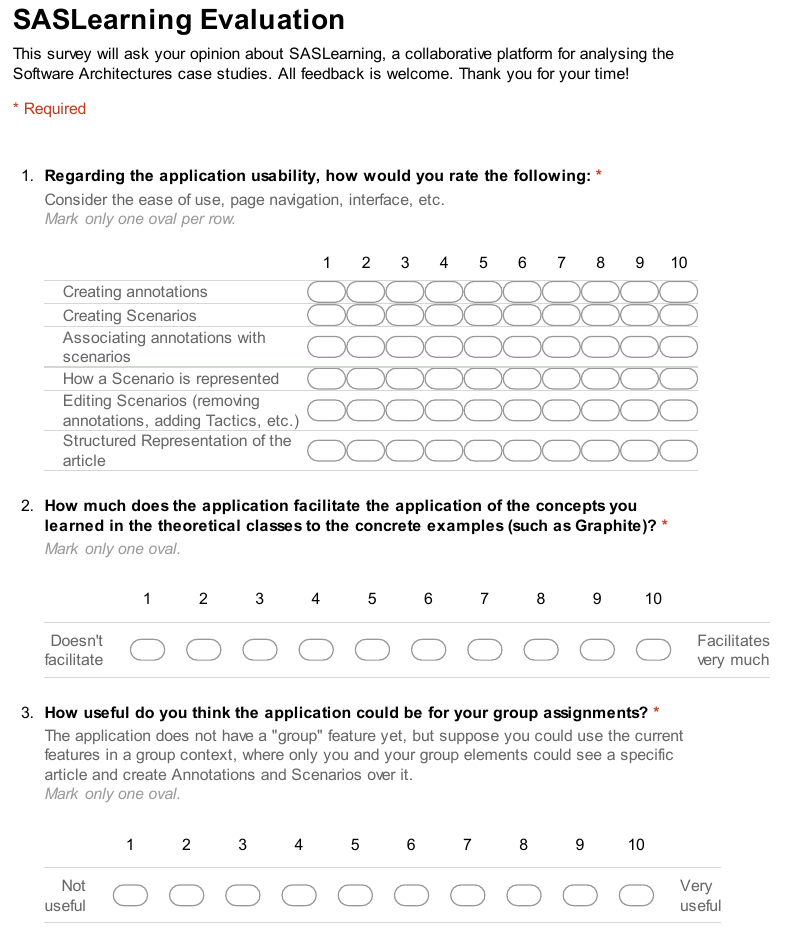
\includegraphics[scale=0.6]{images/survey3}
\end{figure}

\begin{figure}
\centering
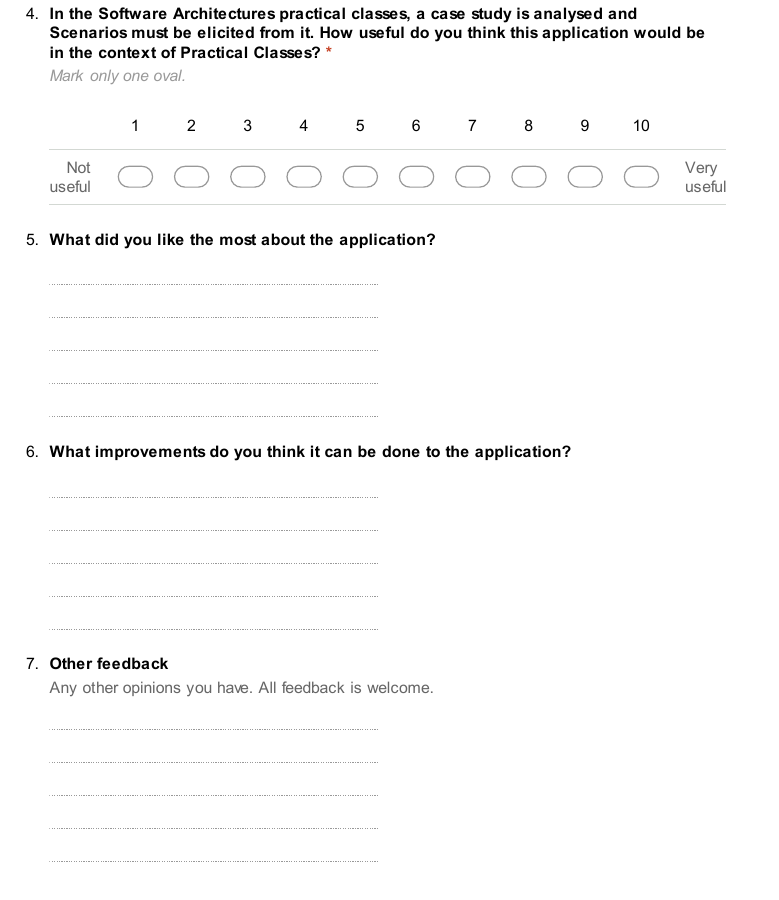
\includegraphics[scale=0.6]{images/survey4}
\end{figure}

%!TEX root = ../dissertation.tex

\chapter{Appendix B - Survey Results}
\label{appendix:appendix_b}

\textbf{Regarding the application usability, how would you rate the following:}
\begin{table}[h]
\centering
\scriptsize
\begin{tabular}{|c|c|c|c|c|c|c|}
    \hline
     \textbf{Participants} & \parbox[c][1cm]{1.5cm}{\textbf{Creating} \\ \textbf{Annotations}} & \parbox[c][1cm]{1.5cm}{\textbf{Creating}\\ \textbf{Scenarios}} & \parbox[c][1cm]{3cm}{\textbf{Associating Annotations} \\ \textbf{with Scenarios}} & \parbox[c][1cm]{2cm}{\textbf{How a Scenario} \\ \textbf{is represented}} & \parbox[c][1cm]{1.5cm}{\textbf{Editing}\\ \textbf{Scenarios}} & \parbox[c][1cm]{2cm}{\textbf{Structured} \\ \textbf{Representation}}\\ \hline
     Participant \#1 & 7 &	9 &	8 & 5 & 4 & 6\\ \hline
	Participant \#2 & 4 & 9 & 1 0 & 7 & 6 & 5\\ \hline
	Participant \#3 & 10 & 10 & 10 & 9 & 9 & 9\\ \hline
	Participant \#4 & 10 & 8 & 8 & 7 & 9 & 7\\ \hline
	Participant \#5 & 10 & 8 & 7 & 8 & 8 & 6\\ \hline
\end{tabular}
\end{table}

\textbf{Application Usefulness:}	
\begin{table}[h]
\centering
\scriptsize
\begin{tabular}{|c|c|c|c|}
    \hline
     \textbf{Participants} & \parbox[c][2cm]{5cm}{\textbf{How much does the application facilitate the application of the concepts you learned in the theoretical classes to the concrete examples (such as Graphite)?}} & \parbox[c][2cm]{3cm}{\textbf{How useful do you think the application could be for your group assignments?}} & \parbox[c][2cm]{3cm}{\textbf{How useful do you think this application would be in the context of Practical Classes?}} \\ \hline
     Participant \#1 & 9 & 9 & 9\\ \hline
Participant \#2 & 8 & 10 & 10\\ \hline
Participant \#3 & 10 & 9 & 10\\ \hline
Participant \#4 & 7 & 7 & 7\\ \hline
Participant \#5 & 7 & 9 & 9\\ \hline
\end{tabular}
\end{table}

\begin{table}[h]
\begin{flushleft}
\textbf{Opinions:} \\
\end{flushleft}

\centering
\scriptsize
\begin{tabular}{|c|c|c|c|}
    \hline
     \textbf{Participants} & \parbox[c][2cm]{2cm}{\textbf{What did you like the most about the application?}} & \parbox[c][2cm]{4cm}{\textbf{What improvements do you think that can be done to the application?}} & \parbox[c][2cm]{4cm}{\textbf{Other feedback}} \\ \hline
Participant \#1 & \parbox[c][2cm]{2cm}{It provides a quick and convenient way of constructing scenarios}& \parbox[c][2cm]{4cm}{There should be a way to "view" the scenario itself, with the diagram that is showed in the lectures. Also, the system needs to be more intuitive, particularly when it comes to selecting sentences for the scenarios} &\parbox[c][2cm]{4cm}{ Would it be possible to view the most common options for each part (stimulus/response/etc.) once you've selected what type of scenario it is (availability/performance/etc.)?} \\ \hline
Participant \#2 & \parbox[c][5cm]{2cm}{I liked most how easy it was to create and edit scenarios} & \parbox[c][2cm]{4cm}{I had trouble when trying annotate a sequence of letters when that sequence overlapped with another annotation. For example, I added a long sequence for the stimulus but then I wanted to use a subsequence of that sequence in the scenario description. I dont remember correctly, but I think I also couldn't add more than one entry per type (like stimulus). And also I couldnt add custom hand-made entries? Sometimes the there is no explicit ""response"", but we can write it and justify it with some part of the text"}  & \parbox[c][2cm]{4cm}{I think this kind of application can be used in other domains. For example it could be used to create character profiles from a narrative book, etc...} \\ \hline
Participant \#3 & \parbox[c][2cm]{2cm}{It is possible for different people to analyze the same document, and its easy to use.} & \parbox[c][2cm]{4cm}{Support sharing files with different groups.} & N/A \\ \hline
Participant \#4 & \parbox[c][2cm]{2cm}{The annotation method} & \parbox[c][2cm]{4cm}{Make multiple copies of the article to bee only seen by each group so that one group doesn't get confused or get influenced by others.} & \parbox[c][2cm]{4cm}{Good luck with the rest of the project!} \\ \hline
Participant \#5 & \parbox[c][2cm]{2cm}{It is extremely easy and intuitive to make annotations, just like on paper.} & \parbox[c][6cm]{4cm}{When adding a tactic, only the tactics presented in the book 'Software Architecture in Practice' are available. I think it could be useful if the user could add new tactics instead of just selecting one of those. The menu bar could be improved by placing there buttons for the main application functionalities. For example, the 'View Structured Representation' link that appears just below the menu bar could be placed on the menu bar instead.An useful functionality could be generating a graphical representation of the scenarios, like those ones on the book with the artifact and the arrows. Another useful (yet difficult to implement, perhaps) functionality would be the possibility to upload new case studies to use in the application.} & Nice work :) \\  \hline		
\end{tabular}
\end{table}



% Glossary and Acronym List
\if\includeGlossary 1
\printglossary
\fi

\end{document}
